%% Standalone figure: wavefunction sampled into an array.
%% Compile with pdflatex; QM.tex loads the resulting PDF with \includegraphics.
\documentclass[11pt]{standalone}   % Crops the page to the drawing; 11pt matches the notes
\usepackage{amsmath,amssymb}       % pmatrix and math symbols
\usepackage{tikz}                  % Drawing
\usetikzlibrary{arrows.meta, decorations.pathreplacing} % Arrow tips; curly brace for the spacing label

\begin{document}
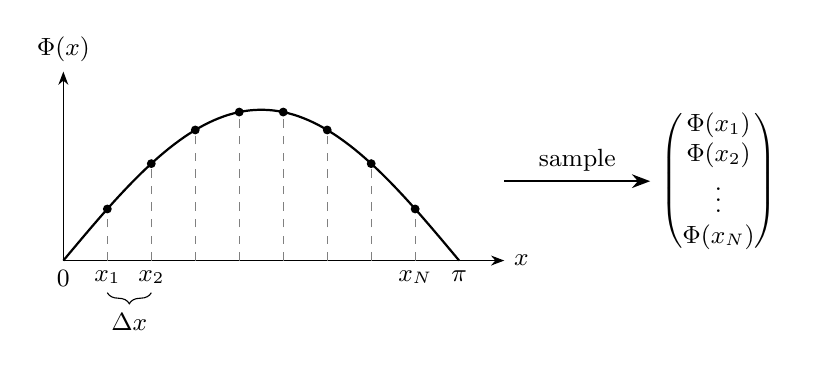
\begin{tikzpicture}[>=Stealth, x=1.6cm, y=2.4cm, font=\small]
    % axes
    \draw[->] (0,0) -- (3.5,0) node[right] {$x$};
    \draw[->] (0,0) -- (0,1.0) node[above] {$\Phi(x)$};
    \node[below] at (0,0) {$0$};
    \node[below] at (pi,0) {$\pi$};
    % continuous wavefunction sqrt(2/pi) sin x
    \draw[thick, domain=0:pi, samples=80] plot (\x, {0.798*sin(\x r)});
    % sampled points x_1 ... x_N
    \foreach \i in {1,...,8} {
        \pgfmathsetmacro{\xi}{\i*pi/9}
        \pgfmathsetmacro{\yi}{0.798*sin(\xi r)}
        \draw[dashed, gray] (\xi,0) -- (\xi,\yi);
        \fill (\xi,\yi) circle (1.6pt);
    }
    \node[below] at ({pi/9},0) {$x_1$};
    \node[below] at ({2*pi/9},0) {$x_2$};
    \node[below] at ({8*pi/9},0) {$x_N$};
    % spacing between neighboring points
    \draw[decorate, decoration={brace, amplitude=4pt, mirror}] ({pi/9},-0.17) -- ({2*pi/9},-0.17) node[midway, below=4pt] {$\Delta x$};
    % array of sampled values
    \node (array) at (5.2,0.42) {$\begin{pmatrix} \Phi(x_1) \\ \Phi(x_2) \\ \vdots \\ \Phi(x_N) \end{pmatrix}$};
    \draw[->, thick] (3.5,0.42) -- (array.west) node[midway, above] {sample};
\end{tikzpicture}
\end{document}
